\chapter{ \toolName}\label{cha:Function}
本研究で試作する\toolName (Mix Visual Regression Test)は、Webページのレイアウトの不具合箇所の発見にかかる時間の削減を目的として、
Webページのレイアウト不具合箇所を強調表示する視覚的回帰テストツール\toolName(Mix Visual Regression Testing)を試作する。
本章では、\toolName の機能と外観について説明する。
% 本研究で用いる「差分箇所」、「変更箇所」、「レイアウトの不具合箇所」を、以下に定義する。
% 本研究で用いる「差分箇所」、「変更箇所」、「レイアウトの副作用箇所」、「レイアウトの不具合箇所」を、以下に定義する。
% 、「比較画像」、「比較HTMLコード」、「テスト画像」、「テストHTMLコード」
\toolName は、以下の3つを強調表示する機能を持つ。
\begin{itemize}
    \item 差分箇所:\\
          変更前後のWebページの画像を比較して、変更前のWebページから削除された範囲と、
          変更後のWebページに追加された範囲。
    \item 変更箇所:\\
          変更前後のWebページのHTMLコードを比較して、HTMLコードにおけるbody要素内の変更とstyle要素内の変更のどちらか、
          または両方が適用された画面要素の範囲。
          本研究では、変更箇所を意図的なレイアウトの差分の範囲とみなす。
    \item レイアウトの不具合箇所:\\
          差分箇所から、意図的なレイアウトの差分の範囲であるHTMLコードの変更箇所を除いた、
          レイアウトの不具合の範囲。
\end{itemize}
% \begin{itemize}
%       \item 差分箇所:\\
%             Webページの変更前画像とWebページの変更後画像を比較して、
%             変更前のWebページから削除された画面要素と変更後のWebページに追加された画面要素。
%       \item 変更箇所:\\
%             変更前後のWebページのHTMLコードを比較して、
%             HTMLコードにおけるbody要素内の変更とstyle要素内の変更のどちらか、
%             または両方の変更が適用された画面要素。
%       \item レイアウトの不具合箇所:\\
%             Webページの変更前画像と変更後画像で、変更箇所によって、
%             HTMLコードを変更していない画面要素にレイアウトの変更があった画面要素。
%             % \item レイアウトの不具合箇所:\\
%             %       レイアウトの副作用箇所のうち、画面要素のはみ出し、重なりがあった画面要素。
%             % \item 比較画像:\\
%             %       視覚的回帰テストにおいて、比較対象とするWebページの画像。
%             % \item 比較HTMLコード:\\
%             %       視覚的回帰テストにおいて、比較対象とするWebページのHTMLコード。
%             % \item テスト画像:\\
%             %       視覚的回帰テストにおいて、テスト対象とするWebページの画像。
%             % \item テストHTMLコード:\\
%             %       視覚的回帰テストにおいて、テスト対象とするWebページのHTMLコード。      
% \end{itemize}

\toolName は、テスト対象のWebページのURLを入力とする。
なお、入力対象とするWebページは、\ref{sec:target_images}節で述べた条件をすべて満たすものとする。
出力は、\ref{subsec:MixVRT_IO}節で後述する8つのPNG形式の画像を閲覧できるWebページである。
\section{\toolName 使用時の流れ}
Webページを作成している開発者が\toolName を使用する際の流れを、以下に示す。
\begin{enumerate}
    \item コマンドライン上で「\$ make test URL=“WebページのURL”」を実行し、初期設定(\ref{subsec:MixVRT_preparation}節で後述)を行う。
    \item WebページのHTMLコードの変更を行う。
    \item コマンドライン上で「\$ make test URL=“WebページのURL”」を実行し、視覚的回帰テストを実行する。
    \item Webブラウザ上で「http://localhost:5000/MixVRT\_diff」にアクセスし、テスト結果を確認する。
    \item テスト結果を評価する
          \begin{itemize}
              \item 問題なし:「\$ make save」を実行し、変更後画像と変更後HTMLコードで、それぞれ変更前画像と変更前HTMLコードを更新する。
              \item 問題あり: 変更前、または、変更後のWebページのHTMLコードを修正し、3.に戻る。
                    %   \item 問題あり: 変更後のWebページのHTMLコードをレイアウトの不具合箇所が発生しないように修正し、3.に戻る。
          \end{itemize}
\end{enumerate}


\section{初期設定}\label{subsec:MixVRT_preparation}
開発者は、\toolName による視覚的回帰テストを実行するために初期設定を行う必要がある。
初期設定は、Python3.9.17\cite{Python}が動作するコマンドライン上で、
以下の\toolName の実行コマンドを実行することで行える。
\begin{lstlisting}[label=list:command,frame=none,numbers=none,basicstyle={\normalsize \ttfamily \color[gray]{.15}}]
  $ make test URL="WebページのURL"
 \end{lstlisting}
{\tt URL}には、入力対象とするWebページのURLを指定する。
\par
この初期設定により、視覚的回帰テストを実行するための変更前画像と変更前HTMLコードを
データ管理部のbase\_dirディレクトリ(表\ref{tb: base_dir_data}を参照)に保持する。
2回目以降の実行は、変更後画像と変更後HTMLコードをデータ管理部のbase\_dirディレクトリに保持し、
変更前画像と変更後画像との比較、変更前HTMLコードと変更後HTMLコードとの比較を行い、視覚的回帰テストを実行する。

\section{入出力}\label{subsec:MixVRT_IO}
初期設定(\ref{subsec:MixVRT_preparation}節を参照)を行った開発者は、
テスト対象とするWebページのURLを入力として\toolName の実行コマンド(\ref{subsec:MixVRT_preparation}節を参照)を実行することで、
\toolName による視覚的回帰テストを実行できる。
視覚的回帰テストの実行後、\toolName は、以下に示す8つのPNG形式の画像を生成する。
% なお、本研究では、①と②を「変更前後画像」、③と④を「差分箇所変更前後画像」、⑤と⑥を「変更箇所変更前後画像」、
% ⑦と⑧を「不具合箇所変更前後画像」と呼ぶ。
% なお、変更前画像をWebページの変更前画像、テスト対象画像をWebページの変更後画像とする。
% \begin{itemize}
%       \item Webページの変更前画像
%       \item Webページの変更後画像
%       \item 画像比較に基づく差分箇所を、色付きの枠で囲むことで強調表示した、Webページの変更前画像
%       \item 画像比較に基づく差分箇所を、色付きの枠で囲むことで強調表示した、Webページの変更後画像
%       \item HTMLコードの変更に基づく変更箇所を、色付きの枠で囲むことで強調表示した、Webページの変更前画像
%       \item HTMLコードの変更に基づく変更箇所を、色付きの枠で囲むことで強調表示した、Webページの変更後画像
%       \item レイアウトの不具合箇所を、色付きの枠で囲むことで強調表示した、Webページの変更前画像
%       \item レイアウトの不具合箇所を、色付きの枠で囲むことで強調表示した、Webページの変更後画像
% \end{itemize}
\begin{itemize}
    \item 変更前画像:\\
          Webページの変更前画像
    \item 変更後画像:\\
          Webページの変更後画像
    \item 差分箇所変更前画像:\\
          変更により削除された範囲を、赤枠で囲むことで強調表示した、Webページの変更前画像
    \item 差分箇所変更後画像:\\
          変更により追加された範囲を、緑枠で囲むことで強調表示した、Webページの変更後画像
    \item 変更箇所変更前画像:\\
          変更により削除された画面要素の範囲を、赤枠で囲むことで強調表示した、Webページの変更前画像
    \item 変更箇所変更後画像:\\
          変更により追加された画面要素の範囲を、緑枠で囲むことで強調表示した、Webページの変更後画像
    \item 不具合箇所変更前画像:\\
          レイアウトの不具合箇所のうち、HTMLコードに基づいて削除されていない範囲を、赤枠で囲むことで強調表示した、Webページの変更前画像
    \item 不具合箇所変更後画像:\\
          レイアウトの不具合箇所のうち、HTMLコードに基づいて追加されていない範囲を、緑枠で囲むことで強調表示した、Webページの変更後画像
\end{itemize}
\toolName は、Flask(\ref{sec:Flask}節を参照)を用いて構築したローカルサーバ上で動作するWebページに、生成した8つの画像を出力し、表示する。
なお、ローカルサーバは、\toolName の環境構築(\ref{sec:MixVRT_env_gen}節を参照)の際に自動で起動する。
\par
開発者は、以下のローカルサーバ上のWebページにアクセスすることで、\toolName が生成した8つの画像を確認できる。
\begin{lstlisting}[label=list:command3,frame=none,numbers=none,basicstyle={\normalsize \ttfamily \color[gray]{.15}}]
    http://localhost:5000/MixVRT_diff
   \end{lstlisting}
なお、\toolName の初期設定時は、変更後画像と変更後HTMLコードが存在せず視覚的回帰テストを行えないため、Webページの変更前画像のみを確認できる。

\section{変更前画像と変更前HTMLコードの更新}\label{subsec:MixVRT_evaluate}
\toolName を用いて変更前後の比較を行い、Webページの更新に問題がないと判断した場合、開発者は下記の実行コマンドを実行する。
これにより、変更後画像と変更後HTMLコードで、それぞれ変更前画像と変更前HTMLコードを更新する。
% 視覚的回帰テストで問題を見つけた場合、開発者はWebページを修正し、\toolName を用いてテストを再度実行して修正が正しいかを検証する。
% 問題がなければ、開発者は下記の実行コマンドを実行する。
% これにより、修正後のテスト再実行時に取得した、変更後画像と変更後HTMLコードを、それぞれ変更前画像と変更前HTMLコードとして更新する。
\begin{lstlisting}[label=list:command2,frame=none,numbers=none,basicstyle={\normalsize \ttfamily \color[gray]{.15}}]
    $ make save
\end{lstlisting}



% また、初回実行時のみにおいて、{\tt URL}には、視覚的回帰テストを行うための比較対象とするWebページのURLを指定する。

% \toolName の初回実行時は、比較対象となるWebページの画像とHTMLコードが存在せず視覚的回帰テストを行えないため、
% 比較対象とするWebページのURLからWebページの画像とHTMLコードの取得のみを行い、処理を終了する。
% \toolName の2回目実行時は、テスト対象とするWebページのURLからWebページの画像とHTMLコードを取得し、
% 比較対象とするWebページの画像とHTMLコードに対して視覚的回帰テストを行う。
% \toolName の3回目以降実行時は、実装の都合上、前回の視覚的回帰テストの結果に関わらず、
% 前回実行時で取得したWebページの画像とHTMLコードを比較対象とし、
% テスト対象とするWebページのURLから取得したWebページの画像とHTMLコードを用いて視覚的回帰テストを行う。
% \par
% \subsection{初期設定}\label{subsec:MixVRT_preparation}
% 開発者は、\toolName による視覚的回帰テストを行うために、以下の初期設定を行う。
% \begin{itemize}
%     \item \toolName の環境構築(\ref{sec:MixVRT_env_gen}節を参照):\\
%           ローカルサーバが起動する。
%     \item \toolName の実行コマンド(\ref{subsec:MixVRT_execution}節を参照)の実行:\\
%           \toolName の初回実行により、視覚的回帰テストを行うための変更前画像と変更前HTMLコードを\toolName に保持する。
% \end{itemize}
% 開発者は、\toolName による視覚的回帰テストを行うために初期設定を行う必要がある。
% 初期設定は、\toolName の実行コマンド(\ref{subsec:MixVRT_execution}節を参照)を実行するだけである。
% \toolName の初回実行により、\toolName による視覚的回帰テストを行うための変更前画像と変更前HTMLコードを
% \toolName のデータ管理部のbase\_dirディレクトリ(\ref{sec:data_admin_section}節で後述)に保持する。



\section{\toolName の外観と機能}\label{sec:MixVRT_Appearance}
\toolName の外観を、図\ref{fig: Appearance}に示す。
\begin{figure}[tp]
    \begin{center}
        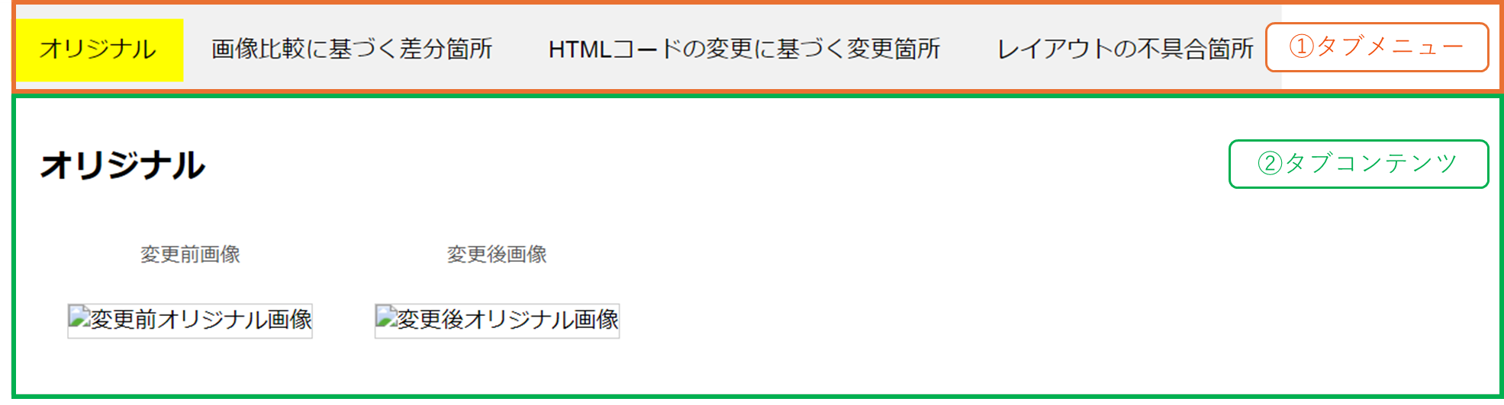
\includegraphics[width=1.0\columnwidth]{image/App.png}
        \caption{\toolName の外観}
        \label{fig: Appearance}
    \end{center}
\end{figure}
\toolName のユーザインタフェースは、以下に示す4つのタブを持つタブメニューと、各タブに対応するタブコンテンツからなる。
なお、以下の数字は、図\ref{fig: Appearance}中の数字と対応している。
\begin{itemize}
    \item[①] タブメニュー
          \begin{itemize}
              \item オリジナル表示
              \item 画像比較に基づく差分箇所表示
              \item HTMLコードの変更に基づく変更箇所表示
              \item レイアウトの不具合箇所表示
          \end{itemize}
    \item[②] タブコンテンツ
\end{itemize}
\par
\toolName の実行コマンド(\ref{list:command}節を参照)を一度も実行していない場合、
図\ref{fig: Appearance}のように、各表示タブにWebページの変更前画像と変更後画像を表示しない。
\par
以降、各タブを選択した際に、表示するタブコンテンツの外観と機能について説明する。

\subsection{オリジナル表示}\label{subsec:original_tab}
オリジナル表示は、「変更前画像」と「変更後画像」を左右に並べて表示する。
オリジナル表示の外観を、図\ref{fig: Appearance_original_tab}に示す。
\begin{figure}[tp]
    \begin{center}
        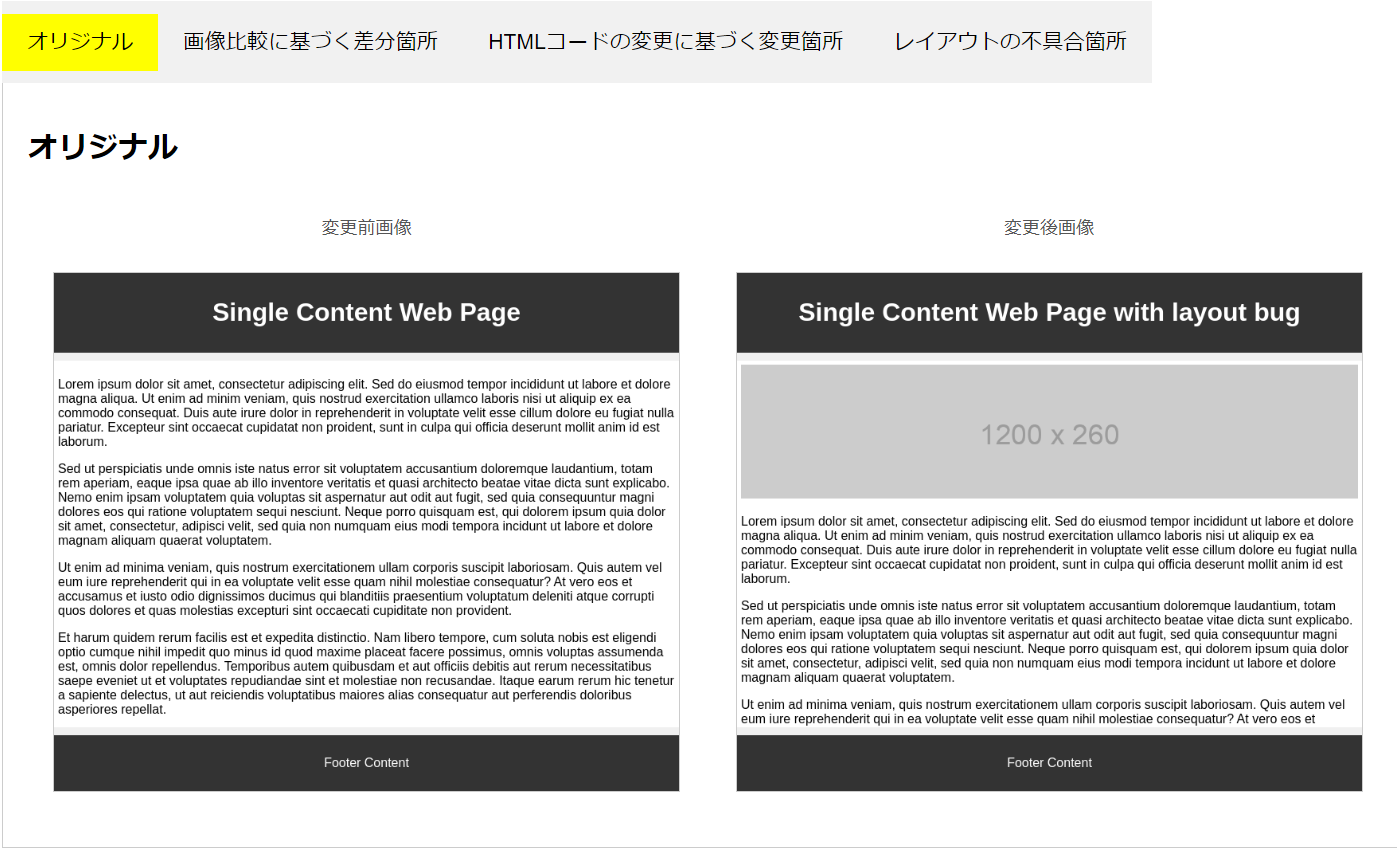
\includegraphics[width=1.0\columnwidth]{image/new_original.png}
        \caption{オリジナル表示の外観}
        \label{fig: Appearance_original_tab}
    \end{center}
\end{figure}
なお、\toolName の初回起動時や変更時は、初期画面として、オリジナル表示を表示する。
ここでは、Webページの変更前後の画像を確認できる。

\subsection{画像比較に基づく差分箇所表示}\label{subsec:images_tab}
画像比較に基づく差分箇所表示は、「差分箇所変更前画像」と「差分箇所変更後画像」を左右に並べて表示する。
画像比較に基づく差分箇所表示の外観を、図\ref{fig: Appearance_images_tab}に示す。
\begin{figure}[tp]
    \begin{center}
        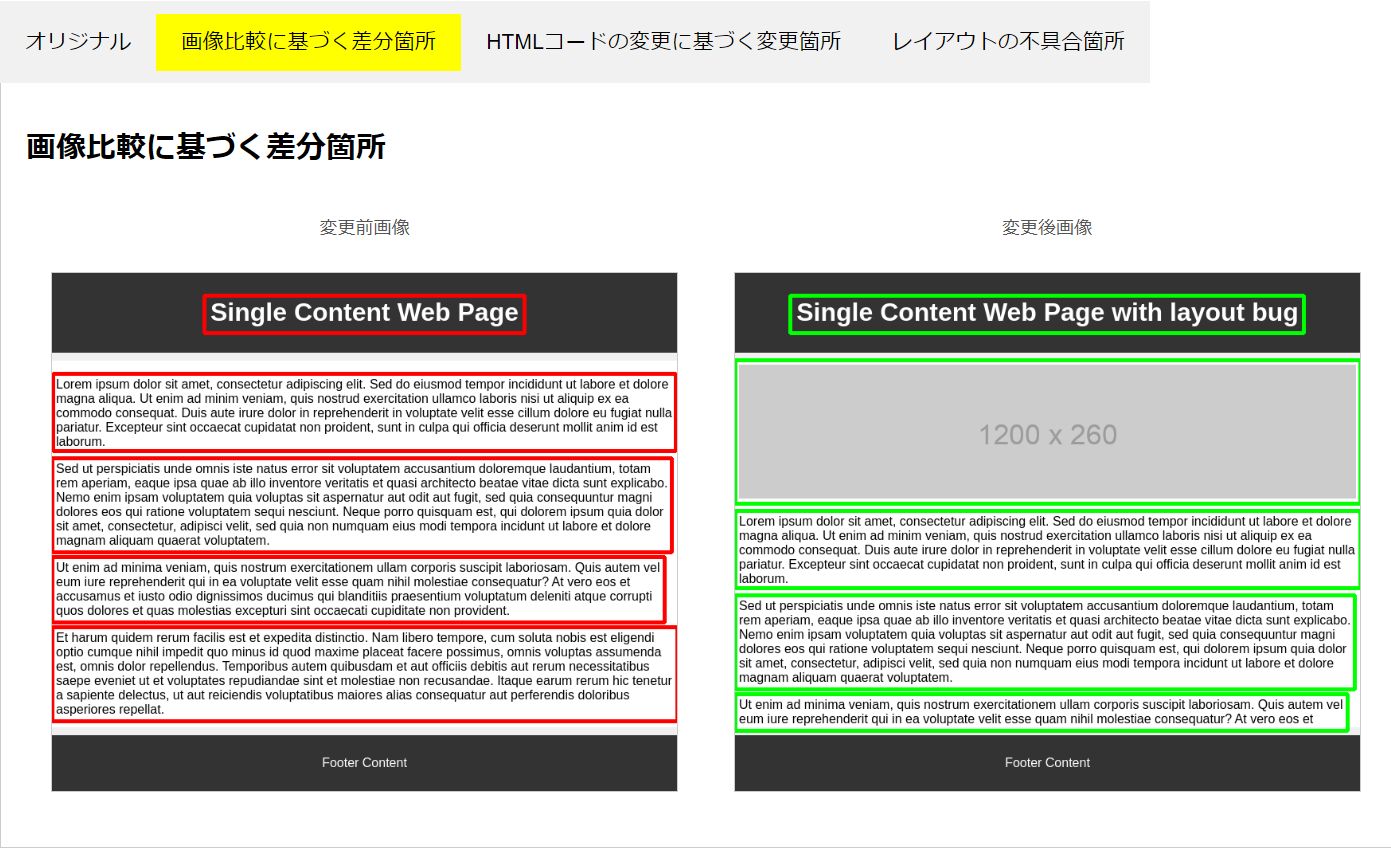
\includegraphics[width=1.0\columnwidth]{image/new_img.png}
        \caption{画像比較に基づく差分箇所表示の外観}
        \label{fig: Appearance_images_tab}
    \end{center}
\end{figure}
削除された範囲は変更前画像上に赤枠で囲むことで強調表示し、追加された範囲は変更後画像上に緑枠で囲むことで強調表示する。
ここでは、変更前後のWebページでレイアウトの差分箇所が生じた範囲を確認できる。

\subsection{HTMLコードの変更に基づく変更箇所表示}\label{subsec:html_tab}
HTMLコードの変更に基づく変更箇所表示は、「変更箇所変更前画像」と「変更箇所変更後画像」を左右に並べて表示する。
HTMLコードの変更に基づく変更箇所表示の外観を、図\ref{fig: Appearance_html_tab}に示す。
\begin{figure}[tp]
    \begin{center}
        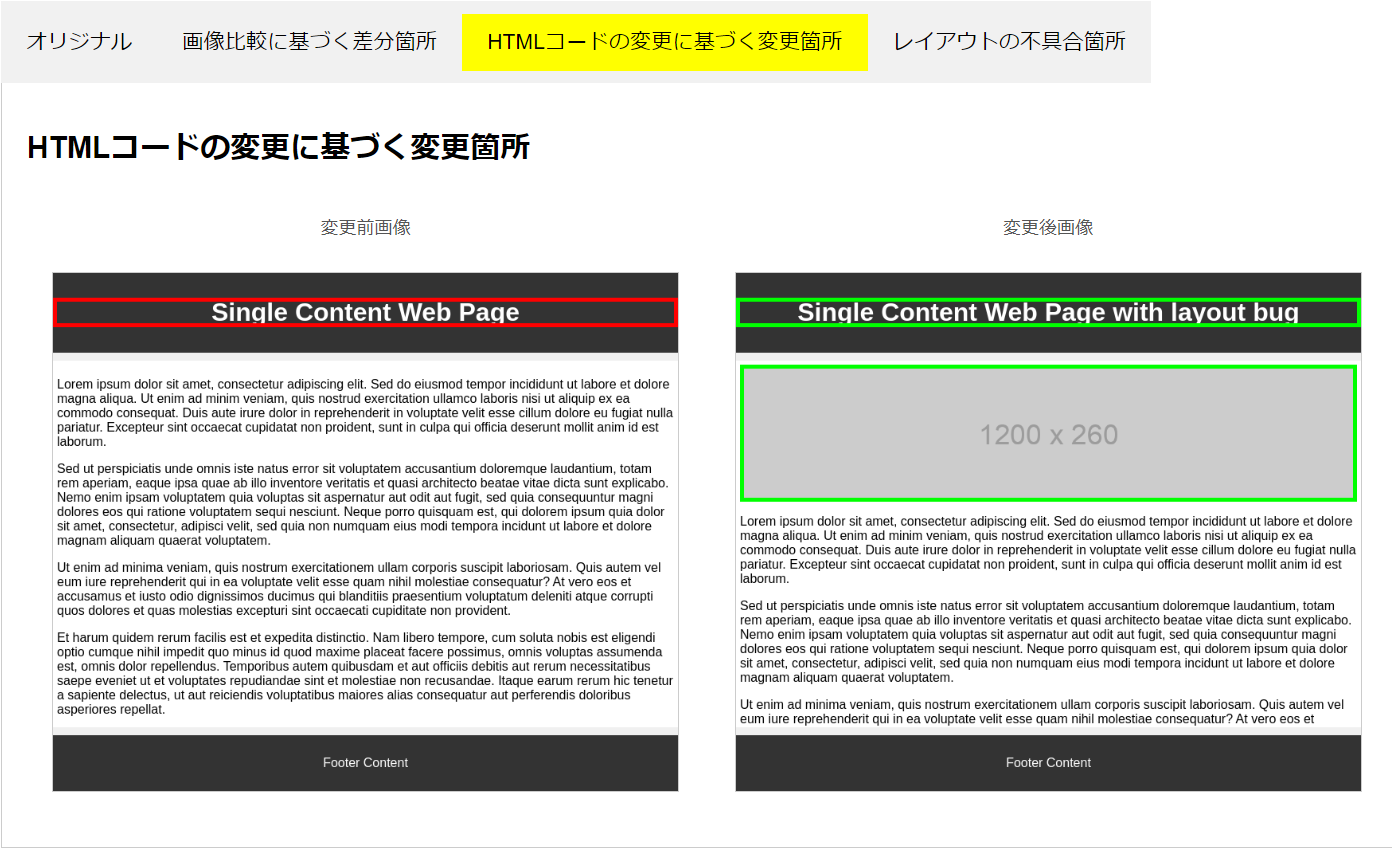
\includegraphics[width=1.0\columnwidth]{image/new_html.png}
        \caption{HTMLコードの変更に基づく変更箇所表示の外観}
        \label{fig: Appearance_html_tab}
    \end{center}
\end{figure}
削除された画面要素の範囲は変更前画像上に赤枠で囲むことで強調表示し、追加された画面要素の範囲は変更後画像上に緑枠で囲むことで強調表示する。
ここでは、図\ref{fig: Appearance_images_tab}における差分箇所から、開発者が変更したHTMLコードに基づく変更箇所のみを確認できる。
% ここでは、変更前後のWebページで開発者が意図した、または意図しないHTMLコードの変更による変更箇所を目視で確認できる。

\subsection{レイアウトの不具合箇所表示}\label{subsec:subeffect_tab}
レイアウトの不具合箇所表示は、「不具合箇所変更前画像」と「不具合箇所変更後画像」を左右に並べて表示する。
レイアウトの不具合箇所表示の外観を、図\ref{fig: Appearance_subEffect_tab}に示す。
\begin{figure}[tp]
    \begin{center}
        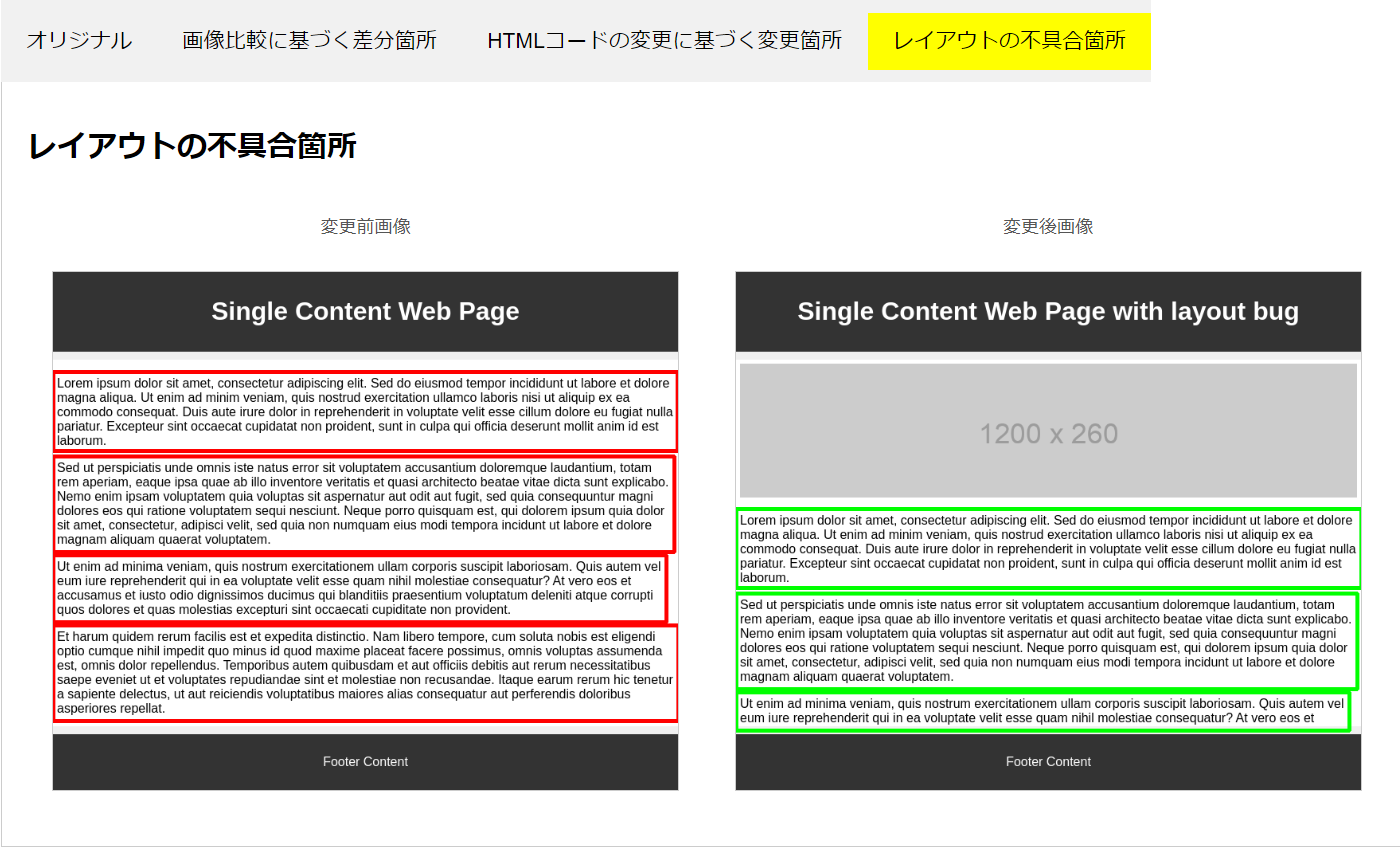
\includegraphics[width=1.0\columnwidth]{image/new_effect.png}
        \caption{レイアウトの不具合箇所表示の外観}
        \label{fig: Appearance_subEffect_tab}
    \end{center}
\end{figure}
ここでは、図\ref{fig: Appearance_images_tab}における差分箇所から特定したレイアウトの不具合箇所のみを確認できる。
図\ref{fig: Appearance_subEffect_tab}の例では、画面要素のはみ出しに該当するレイアウトの不具合箇所を見つけることができる。
\par
図\ref{fig: Appearance_subEffect_tab}における画面要素のはみ出しを、図\ref{fig: out_of_element}に示す。
\begin{figure}[tp]
    \begin{center}
        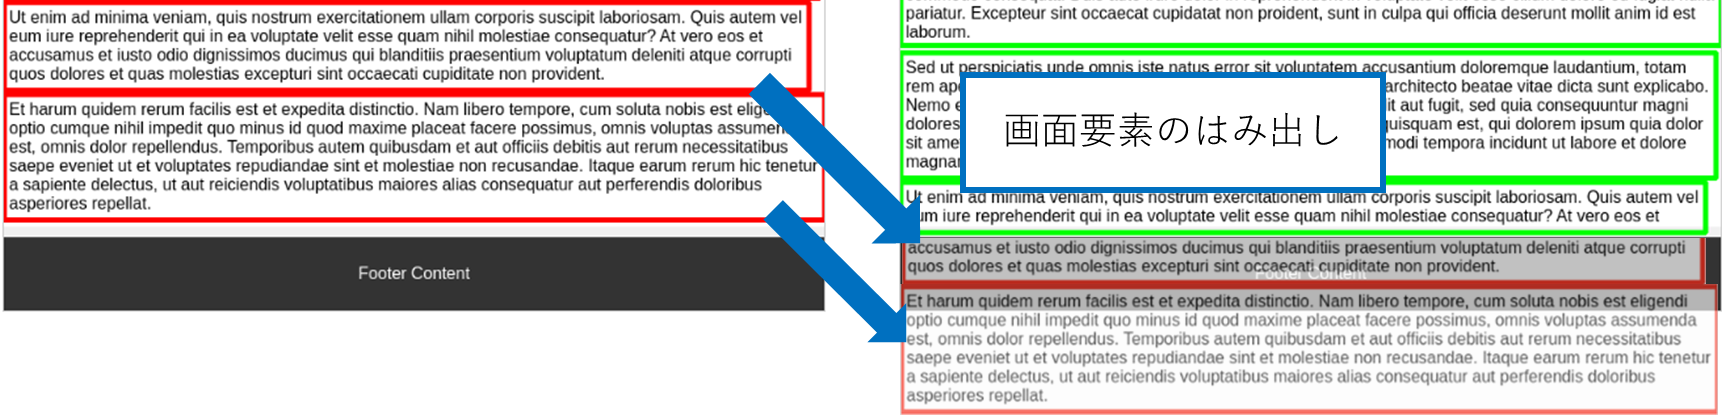
\includegraphics[width=1.0\columnwidth]{image/3_hamidasi_3.png}
        \caption{図\ref{fig: Appearance_subEffect_tab}における画面要素のはみ出し}
        \label{fig: out_of_element}
    \end{center}
\end{figure}
図\ref{fig: out_of_element}内の上の赤枠内と緑枠内のそれぞれのテキストを見比べると、
赤枠内のテキストの上2行目までは緑枠内と同じであるが、赤枠内のテキストの下2行は緑枠内には存在しない。
また、下にある赤枠内のテキストは、変更後の画像には表示されていない。
さらに、図\ref{fig: Appearance_html_tab}より、上の赤枠内のテキストの下2行と下の赤枠内のテキストは
HTMLコードの変更による変更を受けていないと分かるため、削除されたわけではない。
よって、図\ref{fig: out_of_element}の青矢印で示すように、
上の赤枠内のテキスト下2行と下の赤枠内のテキストは、Webページの変更後にコンテナの境界を超えてはみ出した状態になっていると判断できる。
